\section{Introduction}\label{sec:intro}

Enterprise resource planning (ERP) systems are the ledger of record for most
organized economic activity: procurement, payroll, intercompany transfer, and
customer settlement all resolve, eventually, into a stream of timestamped
postings between accounts. Financial fraud and money laundering exploit this
same stream, but rarely as an isolated anomalous posting. The characteristic
shapes of laundering and payment fraud -- a receiving account funded by dozens
of unrelated senders, a chain of transfers that closes on itself days later,
a set of near-identical amounts recurring between two parties -- are properties
of \emph{several transactions taken together}, not of any single row in a
table. A model that scores each transaction independently, however strong its
tabular features, is structurally blind to this class of evidence: two
transactions with identical amount, timestamp, and account features can carry
completely different fraud risk depending on what else has moved through the
same accounts. This is the motivating premise for representing ERP data as a
graph -- accounts as nodes, transactions as time-stamped edges -- and for
asking whether the graph's \emph{topology} carries predictive signal that a
transaction-level baseline does not already capture.

That question is easy to ask and, in the graph-based fraud detection
literature, surprisingly rarely answered cleanly. Two problems recur. First,
temporal graph features are leakage-prone in a way ordinary tabular features
are not: a naively implemented graph statistic (an account's total degree, a
cycle-membership flag, a rolling average) computed over a graph built from the
\emph{whole} dataset will, by construction, let a transaction's features
depend on transactions that occur after it in time -- the graph equivalent of
letting a model see tomorrow's newspaper. Second, when a paper reports that
adding graph structure improves a fraud metric, the improvement is frequently
measured against a baseline of unstated or weaker capacity, so the reader
cannot tell whether the gain reflects genuine structural signal or simply a
better-tuned model. This project's own history is a cautionary instance of
both failures at once. An earlier iteration of the pipeline described in this
paper claimed graph topology as its central differentiator; on audit, its own
feature-importance output showed every topology feature scoring effectively
zero gain importance, while a top-ranked feature turned out to be the time
until the \emph{next} transaction -- future information leaking directly into
a past transaction's row. Its headline accuracy numbers were consequently
uninterpretable. Rebuilding the pipeline so that this failure mode is
structurally impossible, and then running the first fair test of the original
question, is the starting point of this paper.

\subsection{The Scientific Claim}

We deliberately narrow the question this paper answers. It would be easy to
frame the contribution as a real-time fraud-monitoring platform for ERP
systems -- and the system sections later in this paper do describe a working
console that ingests postings, computes features online, and surfaces
explained alerts. But a working system is a
demonstration, not evidence of the platform's founding hypothesis, and this
paper treats it accordingly: as the \emph{vision} the architecture is built
toward, not the \emph{proof} it is asked to supply. The proof this paper
commits to is narrower, falsifiable, and stated once, precisely, here:

\begin{quote}
\emph{Temporal graph topology features add predictive value over a strong
tabular baseline, measured without leakage.}
\end{quote}

Every other claim in this paper -- about the streaming architecture, the
synthetic data generator, the production console, the explanation layer -- is
in service of being able to answer that question honestly, on a real dataset,
without the answer being pre-determined by how the experiment was built. We
committed, before running the decisive experiment, to reporting whatever it
showed, including a negative result on any of the four datasets tested. As
quantified later in this paper, the honest answer turns out to be
conditional: topology helps substantially where
the tabular baseline has headroom and fraud leaves a structural trace, is
uninformative where the baseline is already near-saturated by amount alone,
and on the one dataset with genuinely thin ERP-style graph structure and very
few labeled test frauds, topology measurably \emph{hurts} the full model. We
report that last result plainly rather than omitting it, because a paper that
sets out to test whether topology helps is not entitled to discard the trial
where it did not.

\subsection{Leakage as a Design Constraint, Not a Post-hoc Check}

The central engineering response to the leakage failure above is a streaming
computation model applied uniformly to every topology feature, rather than a
leakage \emph{test} applied after the fact to features computed some other
way. Transactions are processed in a single pass, ordered by timestamp with
ties broken by a fixed, arbitrary total order over the input rows. Let
$\tau_1, \tau_2, \dots, \tau_n$ denote this processing order and let $G_i$
denote the graph state after transactions $\tau_1, \dots, \tau_i$ have been
inserted, with $G_0 = \emptyset$. For every transaction $\tau_i$, the engine
enforces

\[
\phi(\tau_i) = f\bigl(G_{i-1}\bigr), \qquad\text{then}\qquad G_i \leftarrow G_{i-1} \cup \{\tau_i\},
\]

\noindent i.e., the feature vector $\phi(\tau_i)$ is computed and persisted
against the graph state that excludes $\tau_i$ itself and everything after
it, and only \emph{then} is $\tau_i$ inserted. We refer to this as the
\emph{read-then-insert invariant}. It is not merely a coding convention: a
structural property that once a feature vector is written it is provably a
function of $\tau_i$'s strict causal past means a later transaction can be
proven, not merely assumed, to be unable to alter an earlier transaction's
features. A later section of this paper formalizes the leakage taxonomy this
invariant closes off, and the accompanying automated regression test --
adversarially scrambling the order of not-yet-processed transactions and
asserting that no already-computed feature changes -- has stayed green
through every stage of this project's rebuild. Figure~\ref{fig:pipeline}
sketches the resulting pipeline end to end, including the point at which the
deployed system diverges from the research configuration used to establish
the scientific claim above, elaborated fully in the system description
later in this paper.

\begin{figure}[t]
\centering
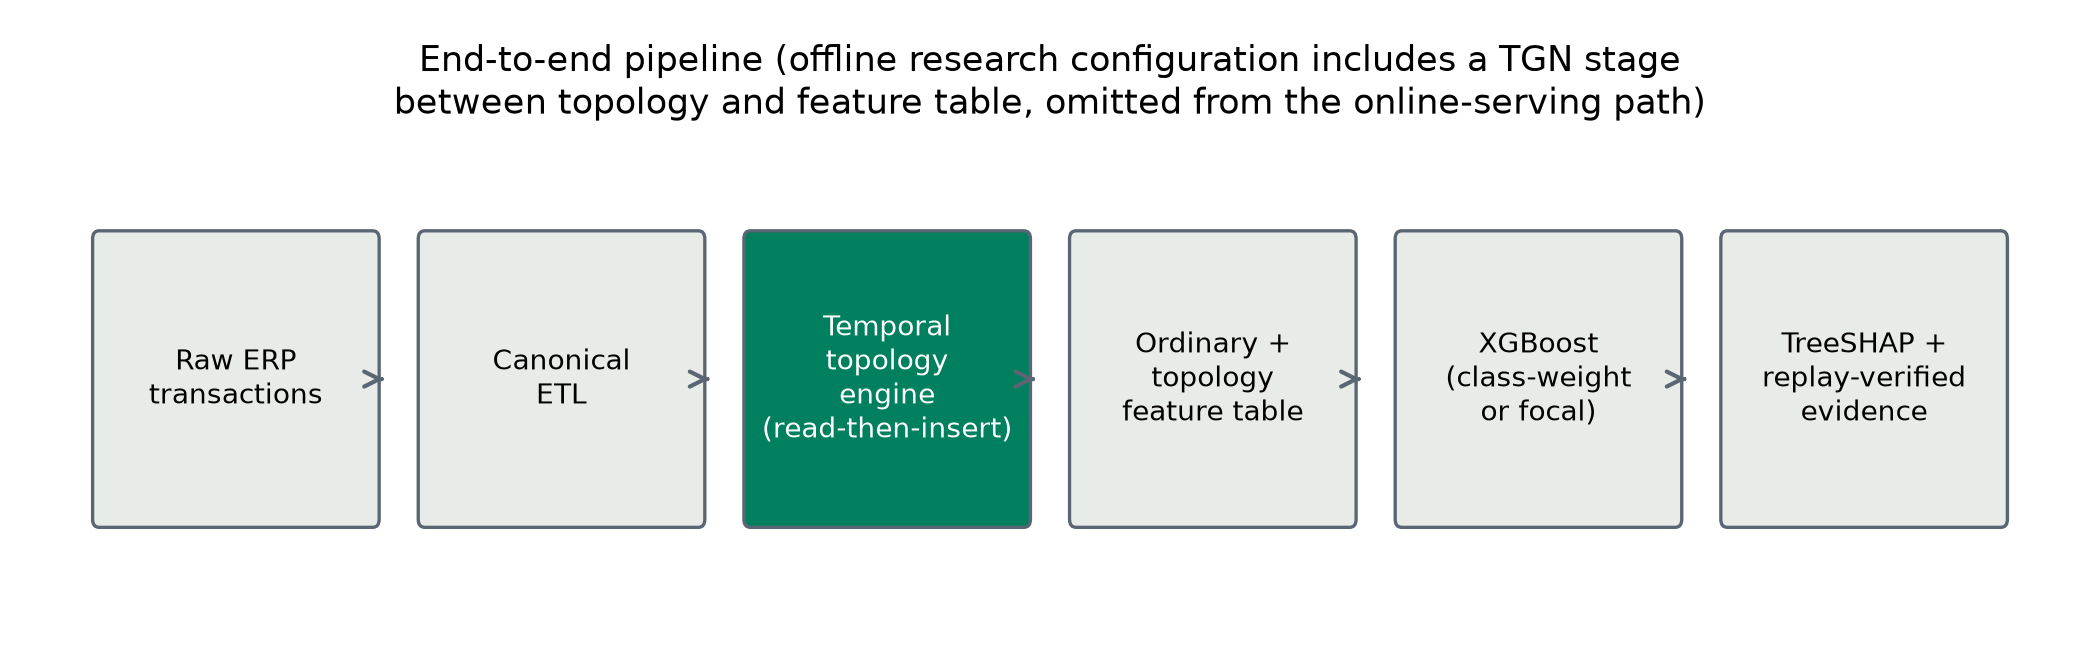
\includegraphics[width=\columnwidth]{figures/pipeline_overview.png}
\caption{End-to-end pipeline. Raw ERP transaction feeds are cleaned into a
canonical accounts/transactions schema, assembled into a temporal shadow
graph, and passed through the streaming topology engine under the
read-then-insert invariant, so that a feature is provably a function only of
transactions strictly earlier in processing order. The resulting feature
table (ordinary + topology, with offline-only TGN embeddings added for the
research configuration) feeds a gradient-boosted model; the console layer
attaches a TreeSHAP explanation and a re-derived evidence path to every
alert. The production/online bundle omits the TGN component, since its
learned memory tensor is not persisted for live inference.}
\label{fig:pipeline}
\end{figure}
%% FIGURE TODO: Six-stage left-to-right pipeline diagram: (1) Raw ERP transaction CSVs -> (2) ETL to canonical accounts+transactions schema -> (3) Temporal shadow graph (Neo4j, visualization/demo path only, never load-bearing for scoring) -> (4) Streaming topology engine, with a callout box reading "for transaction i: read features from G_{i-1}, THEN insert transaction i into G_i" -> (5) Feature table (ordinary + topology [+ TGN embeddings, offline research path only]) -> (6a) Offline XGBoost champion (topology+TGN, research/ablation use only, not servable) and (6b) Online XGBoost bundle (ordinary+topology only, actually deployed) -> forensic console alert card showing SHAP attribution bars tagged by feature family (ordinary/topology/topology-amount-derived/tgn) plus a reconstructed evidence path (cycle or fan-in) redrawn from the graph at scoring time.

\subsection{Contributions}

This paper makes five contributions, listed in the order the paper
substantiates them:

\begin{enumerate}
\item \textbf{A leakage-free streaming topology engine with a formal
read-then-insert invariant.} Every one of the engine's structural detectors
(in-/out-degree fan-in and fan-out, cycle membership and amount-conserving
cycle features, and recurring near-equal-amount ``lapping'' features) is
computed under the invariant above and guarded by an automated,
order-scrambling regression test, rather than validated only by an
after-the-fact audit.

\item \textbf{A rigorous within-dataset ablation across four heterogeneous
datasets.} The same feature engine, model family, and evaluation protocol are
applied, unchanged, to two independent real-world payment datasets, one real
ERP general-ledger dataset, and one internally generated synthetic dataset
chosen to span a deliberate spectrum of graph structure, from near-tree
(customer-to-merchant only, cycles structurally impossible) to rich,
cyclical, multi-account flows. Reporting the same probe on datasets that
differ this much in how much structure they even contain is itself part of
the evidence: a topology signal that appears only where structure is rich and
vanishes where it is sparse is more credible than one reported on a single
dataset.

\item \textbf{A calibrated synthetic ERP economy generator with an
adversarial realism audit.} To study topology-rich fraud behavior and to
probe whether synthetic data can safely augment real training sets, we build
a seeded, agent-based synthetic ERP economy whose fraud is generated from
criminal goals and evasion behavior rather than from the shapes our own
detectors look for -- avoiding the circularity of grading a detector against
data manufactured to fit it -- and subject it to an independent adversarial
review and a realism battery before using it for anything beyond sanity
checks.

\item \textbf{A production system that serves the leakage-free feature
computation online.} The same streaming engine that produces the research
feature table also backs a running ERP application and forensic audit
console, computing ordinary and topology features on live postings under the
identical read-then-insert invariant. We are explicit throughout this paper
about a consequential asymmetry: the strongest \emph{offline} research
configuration additionally includes learned temporal-graph-network (TGN)
embeddings, but the TGN's per-account memory state is not persisted, is not
guaranteed bit-reproducible across machines even under a fixed random seed
(quantified later in this paper), and is therefore
never part of what is actually served online. Every PR-AUC figure in this
paper is labeled as belonging to one of two distinct models -- the
\emph{offline champion} (topology and, where used, TGN) or the
\emph{deployed online bundle} (ordinary and topology only) -- and the two are
never conflated.

\item \textbf{Full transparency, including negative and null results.}
Alongside the positive result, we report, without softening: a dataset on
which the full model's topology addition measurably reduces PR-AUC; a
dataset whose tabular baseline is already so strong that the marginal
comparison is close to uninformative; an ablation study that is single-seed
and therefore silent on whether a small positive lift is signal or noise; a
headline structural-motif family (cycle detection) that contributes
negligible gain importance on most of the datasets studied despite being the
project's original motivating idea; and a synthetic-data augmentation
experiment whose main finding is that naive augmentation \emph{degrades}
real-data performance, with only a narrower, different transfer claim holding
up.
\end{enumerate}

\subsection{Preview of Findings}

Across the two real payment-network datasets and the real ERP ledger dataset
evaluated in the final, multi-seed model comparison, the picture is genuinely
mixed, not uniformly positive. On the sparse, customer-to-merchant payment
dataset -- structurally incapable of containing true multi-hop cycles --
adding hand-crafted topology features raises test PR-AUC from a
$0.7870 \pm 0.0700$ ordinary-feature baseline to $0.9319 \pm 0.0017$, and the
fully tuned champion configuration reaches $0.9364 \pm 0.0015$ with perfect
precision at the top 100 alerts. On the anti-money-laundering simulation
dataset, whose ordinary-feature baseline already reaches
$0.9920 \pm 0.0026$ PR-AUC, adding topology reaches a ceiling of
$1.0000 \pm 0.0000$ -- a result we flag, not celebrate, as an artifact of an
already-saturated baseline rather than evidence of a large structural effect;
the informative signal on this dataset lives in an amount-blind probe
reported later, not in this marginal comparison. On the real,
university-published SAP general-ledger dataset, the honest result runs the other way:
the ordinary-feature baseline reaches $0.1581 \pm 0.0129$ PR-AUC, and adding
topology \emph{lowers} it to $0.0717 \pm 0.0095$; only after a full
hyperparameter search and a change of imbalance mechanism does the final
champion claw back to $0.1557 \pm 0.0717$, statistically indistinguishable
from the ordinary baseline it started from. This dataset carries only 25
labeled test frauds, and we treat the result as underpowered rather than
disproving the hypothesis outright -- but we do not discard it, and we do not
let the two datasets where topology clearly helps stand in for a result that,
on this one, it measurably did not. We return to all three results with full
detail, confidence caveats, and feature-level attribution later in this
paper.

\subsection{Paper Organization}

Section~\ref{sec:related} situates this paper in the graph-based fraud
detection, class-imbalance, temporal graph network, continuous-auditing, and
explainability literatures, and argues that this paper's central gap-filling
contribution is methodological -- an explicit leakage taxonomy and a
same-architecture, multi-dataset ablation -- rather than a new graph
architecture. Later sections (not assigned to this document) develop the
leakage taxonomy and its automated guard in full, describe the four
evaluation datasets and the synthetic generator's realism audit, detail the
streaming architecture and the production ERP and forensic console, report
the ablation and augmentation experiments with complete confidence
accounting, and close with the explainability layer, limitations, and future
work.

\section{Related Work}\label{sec:related}

This section reviews five bodies of work this paper draws on -- graph-based
fraud and money-laundering detection, class-imbalance learning, temporal
graph networks, continuous auditing and ERP-centric fraud research, and
post-hoc explainability -- and closes by positioning this paper's
contribution against the first of these in particular.

\subsection{Graph-Based Fraud and Anti-Money-Laundering Detection}

The premise that fraud and laundering are relational, not point, phenomena
has produced a substantial and fast-growing graph neural network (GNN)
literature, surveyed broadly by Yuan et al.~\cite{yuan2025survey} for
GNN-based anomaly detection and specifically for financial fraud by Motie and
Raahemi~\cite{motie2024gnn}, whose systematic review taxonomizes
architectures, node/edge representations, and evaluation practices across
the field. Within that space, several recent directions are represented in
the citations this paper draws on. Devi et al.~\cite{devi2025rlgnn} fuse
reinforcement learning with a GNN backbone for real-time fraud detection,
aiming at the same online-scoring setting this paper's production console
targets. Tong et al.~\cite{tong2023financial} and Zhi et
al.~\cite{zhi2025imbalanced} both target the fraud literature's dominant
practical obstacle -- extreme class imbalance -- from the graph side,
combining GNN representations with imbalance-aware learning and,
respectively, an embedding-aware conditional GAN for synthetic minority
generation. Boyapati et al.~\cite{boyapati2025balancer} propose an
architecture-level balancing mechanism (BalancerGNN) rather than a
data-level one. Shi et al.~\cite{shi2026uncertainty} combine spatio-temporal
contrastive representation learning with explicit uncertainty
quantification, addressing a concern this paper shares -- that a bare
point-estimate fraud score is of limited use to an auditor who must decide
how much to trust it. A smaller quantum-computing strand is also
represented: Innan et al.~\cite{innan2024quantum} and Grossi et
al.~\cite{grossi2022mixed} both explore quantum and hybrid quantum-classical
graph learning for fraud classification and feature selection; both are, by
the nature of current quantum hardware, proof-of-concept studies rather than
deployment-scale systems, and we include them here for completeness of the
graph-fraud landscape rather than as a direct comparison point for the
tabular-scale production system this paper describes. Table~\ref{tab:related_gnn}
summarizes the method family and stated focus of each.

\begin{table}[t]
\centering
\small
\caption{Representative recent graph-based approaches to financial fraud and
anti-money-laundering detection cited in this paper.}
\label{tab:related_gnn}
\begin{tabular}{@{}p{0.13\columnwidth}p{0.36\columnwidth}p{0.40\columnwidth}@{}}
\toprule
\textbf{Source} & \textbf{Method family} & \textbf{Stated focus} \\
\midrule
\cite{motie2024gnn} & Systematic review & GNN architectures for financial fraud, taxonomized \\
\cite{yuan2025survey} & Survey & GNN-based anomaly detection broadly, fraud as one application \\
\cite{innan2024quantum} & Quantum GNN & Fraud classification via quantum graph circuits \\
\cite{grossi2022mixed} & Quantum-classical hybrid & Fraud detection with quantum-assisted feature selection \\
\cite{devi2025rlgnn} & RL + GNN fusion & Real-time fraud scoring via RL-guided graph policies \\
\cite{tong2023financial} & GNN + imbalance learning & Transaction-level fraud detection under class skew \\
\cite{zhi2025imbalanced} & Conditional GAN + embeddings & Synthetic minority generation for imbalanced fraud data \\
\cite{boyapati2025balancer} & Balanced GNN architecture & Architecture-level remedy for imbalanced graph classification \\
\cite{shi2026uncertainty} & Contrastive + uncertainty-aware GNN & Spatio-temporal fraud detection with calibrated confidence \\
\cite{wang2023reinforced} & RL causal explainer & Post-hoc causal explanation for GNN predictions \\
\bottomrule
\end{tabular}
\end{table}

What this literature only inconsistently reports, and rarely reports jointly,
is (i) an explicit statement of how a temporal or relational feature's
computation is bounded relative to the timestamp of the transaction it
describes, and (ii) a same-architecture ablation isolating the graph
component's marginal contribution over a tabular baseline of matched
capacity. This paper's own pre-rebuild history is direct evidence that this
omission is not merely academic: without both a formal temporal-computation
invariant and a first-class ablation, a reported gain from adding graph
structure is not distinguishable, from the outside, from a gain produced by
leakage or by an unmatched baseline. We return to this gap in
Section~\ref{sec:related-gap}.

\subsection{Class-Imbalance Learning}

Fraud labels are rare by construction -- across the four datasets used later
in this paper, positive rates range from roughly one in a thousand
transactions to just over one in a hundred -- and imbalance-handling choices
materially affect both accuracy and, importantly, its variance across
training runs. Lin et al.~\cite{lin2017focal} introduce focal loss for dense object
detection, reshaping the standard cross-entropy objective to down-weight
easy, confidently-correct examples so that training gradient is concentrated
on the hard cases; the same reshaping transfers naturally to rare-event
tabular classification and is used later in this paper's own model-selection
protocol, compared head-to-head against simple class weighting under a rule
that the two imbalance mechanisms are never combined within a single
experiment. Zhi et al.~\cite{zhi2025imbalanced}, discussed above, instead address
imbalance at the data level via conditional generative augmentation of the
minority class within a graph-aware embedding space -- a resampling family we
deliberately avoid for structural (as opposed to purely tabular) features,
since interpolating between two graph-derived feature vectors can produce a
combination -- for instance, half of a cycle -- with no physical
transaction-graph realization.

\subsection{Temporal Graph Networks}

Rossi et al.~\cite{rossi2020temporal} introduce Temporal Graph Networks (TGNs): a
memory-augmented architecture that maintains a compact, continuously-updated
state vector per node, updated via a recurrent cell as each new edge (here, a
transaction) is observed, and trained with a self-supervised link-prediction
objective rather than direct supervision on any downstream label. This paper
adopts a TGN, trained self-supervised and hence label-free, as the learned
counterpart to the hand-crafted topology detectors in its offline research
configuration: an account's TGN embedding is read \emph{before} the
transaction that updates it is folded into memory, preserving the same
temporal-ordering discipline used for the hand-crafted features, and the
embedding is deliberately restricted from access to transaction amounts so
that its contribution can be isolated from the model's known amount-driven
signal. Later sections of this paper are explicit, however, that this
paper does not treat the TGN as free to deploy: floating-point
non-determinism in CPU-trained recurrent updates compounds over an
epoch's worth of transactions to the point that TGN-derived embeddings
retrained on the same, fixed random seed but on a different machine are not
bit-reproducible against a previously committed model, and the memory state
itself is not persisted for streaming inference -- both properties that keep
the TGN a research-arm-only component in this paper's accounting, never part
of the production-served model.

\subsection{Continuous Auditing and ERP-Centric Fraud Research}

A parallel, older literature addresses fraud and control failures from the
audit and information-systems side rather than the machine-learning side.
Vasarhelyi et al.~\cite{vasarhelyi2012acceptance} study the acceptance and adoption of
continuous auditing techniques by internal auditors, documenting that
technique sophistication alone does not guarantee organizational uptake --
relevant context for this paper's emphasis on an audit console that surfaces
not just a score but a reconstructed, human-checkable evidence path for every
alert, since an unexplained score is exactly the kind of output that
technique-adoption research finds auditors distrust. Jawad et al.~\cite{jawad2024erp}
review machine-learning-driven optimization of ERP systems broadly, situating
fraud scoring as one of several ML use cases layered on ERP data (alongside
demand forecasting, process mining, and anomaly detection in master data) and
noting that most such deployments remain post-hoc analytics layered outside
the transactional system of record rather than integrated into it --
precisely the gap this paper's production console, built to score
transactions at posting time rather than in a downstream batch job, is meant
to close. Mamakou et al.~\cite{mamakou2024postimplementation} evaluate ERP systems
post-implementation from internal auditors' own perspective, underscoring
that an ERP-adjacent tool's practical value is judged by auditors against
criteria -- traceability, explainability of automated outputs, and
compatibility with existing control frameworks -- that a raw model accuracy
number does not, by itself, satisfy. Together, this literature motivates why
this paper treats the explanation and evidence-reconstruction layer as a
first-class deliverable rather than an add-on to a scoring model.

\subsection{Explainability for Tree and Graph Models}

An accuracy figure, however well validated, does not on its own justify
opening a fraud investigation; the audience for a fraud alert needs to know
\emph{why} a transaction scored highly. Lundberg and Lee~\cite{lundberg2017unified} unify a
family of additive feature-attribution methods under the Shapley-value-based
SHAP framework, providing a game-theoretic, locally accurate decomposition of
a model's output into per-feature contributions. Lundberg et al.~\cite{lundberg2020local}
extend this to TreeSHAP, an algorithm that computes exact (not sampled or
approximated) Shapley values for tree-ensemble models in low-order polynomial
time -- a property this paper relies on directly, since it is a
determining factor, alongside raw predictive accuracy, in this paper's choice
of a gradient-boosted tree ensemble as the final classifier head over an
end-to-end neural alternative: exact, cheap attribution is available for
trees in a way it is not for most deep architectures. On the graph side,
Wang et al.~\cite{wang2023reinforced} propose a reinforcement-learning-based causal
explainer for GNN predictions, targeting a complementary explainability
problem -- explaining which subgraph structure drove a graph model's own
decision, rather than which tabular feature drove a downstream classifier's
decision. This paper's design deliberately sidesteps needing a GNN-native
explainer of that kind for its production scoring path, feeding learned graph
signal into TreeSHAP-explainable tree features rather than explaining a graph
model's decision directly; the graph itself is instead re-rendered for the
auditor as the literal evidence path (the reconstructed cycle or fan-in
structure a given alert is attributed to), verified independently at display
time against the same stored feature state the score was computed from.

\subsection{Positioning of This Work}\label{sec:related-gap}

Read across the sections above, the recurring shape of the gap this paper
targets is consistent. Model novelty in the graph-based fraud literature is
abundant: new architectures, new imbalance-handling mechanisms, new
uncertainty-quantification and explainability layers all appear at a healthy
pace, and the citations above are one small, recent sample of that pace. What
is comparatively scarce, and what this paper is built around supplying, is
methodological accounting for two specific threats to validity that are easy
to state and easy to violate silently: whether a temporal or relational
feature could, even in principle, have depended on information from after
the event it describes, and whether an architecture's graph component is
being compared against a tabular baseline of genuinely matched capacity
rather than a weaker straw-man. Neither threat is exotic -- this paper's own
preliminary iteration fell to both simultaneously, with a future-looking
feature ranked among its most important, before an internal audit caught it
-- and neither is fully addressed by adding a leakage \emph{test} after
model development, since a test can only catch a violation the engineer
thought to check for. The response this paper takes is architectural rather
than remedial: a read-then-insert invariant enforced in the feature engine
itself (Section~\ref{sec:intro}), guarded by an automated regression test
rather than a one-time audit, and a within-dataset, same-architecture
ablation run identically across four structurally different datasets rather
than a single headline comparison. This paper's technical components --
hand-crafted topology detectors, a TGN~\cite{rossi2020temporal},
gradient-boosted trees, focal-loss and class-weight imbalance handling
\cite{lin2017focal}, and TreeSHAP attribution \cite{lundberg2020local} --
are consequently adaptations of established techniques rather than new
architectures in their own right. The contribution is the discipline wrapped
around them, and the willingness, evidenced throughout this paper, to report
what that discipline finds even when it is a negative result on the very
dataset the project's original hypothesis was built to explain.
